% ============================================================
\section{Datos}
\label{sec:datos}
% ============================================================

Se usan dos fuentes. La primera son las salidas de los modelos CMIP6 para la variable \texttt{tos} (TSM, tabla CMOR \texttt{Omon}), obtenidas de la federación ESGF (\emph{Earth System Grid Federation}) y, de forma complementaria, del Copernicus Climate Data Store (CDS). La segunda es ERSSTv5 (\emph{Extended Reconstructed Sea Surface Temperature}, versión~5) de NOAA, descargada de NOAA PSL, que es la referencia observacional única de todo el \emph{pipeline}. La Figura~\ref{fig:cmip6_contribution} muestra la procedencia institucional de los 40 modelos seleccionados.

\begin{figure}[htbp]
\centering
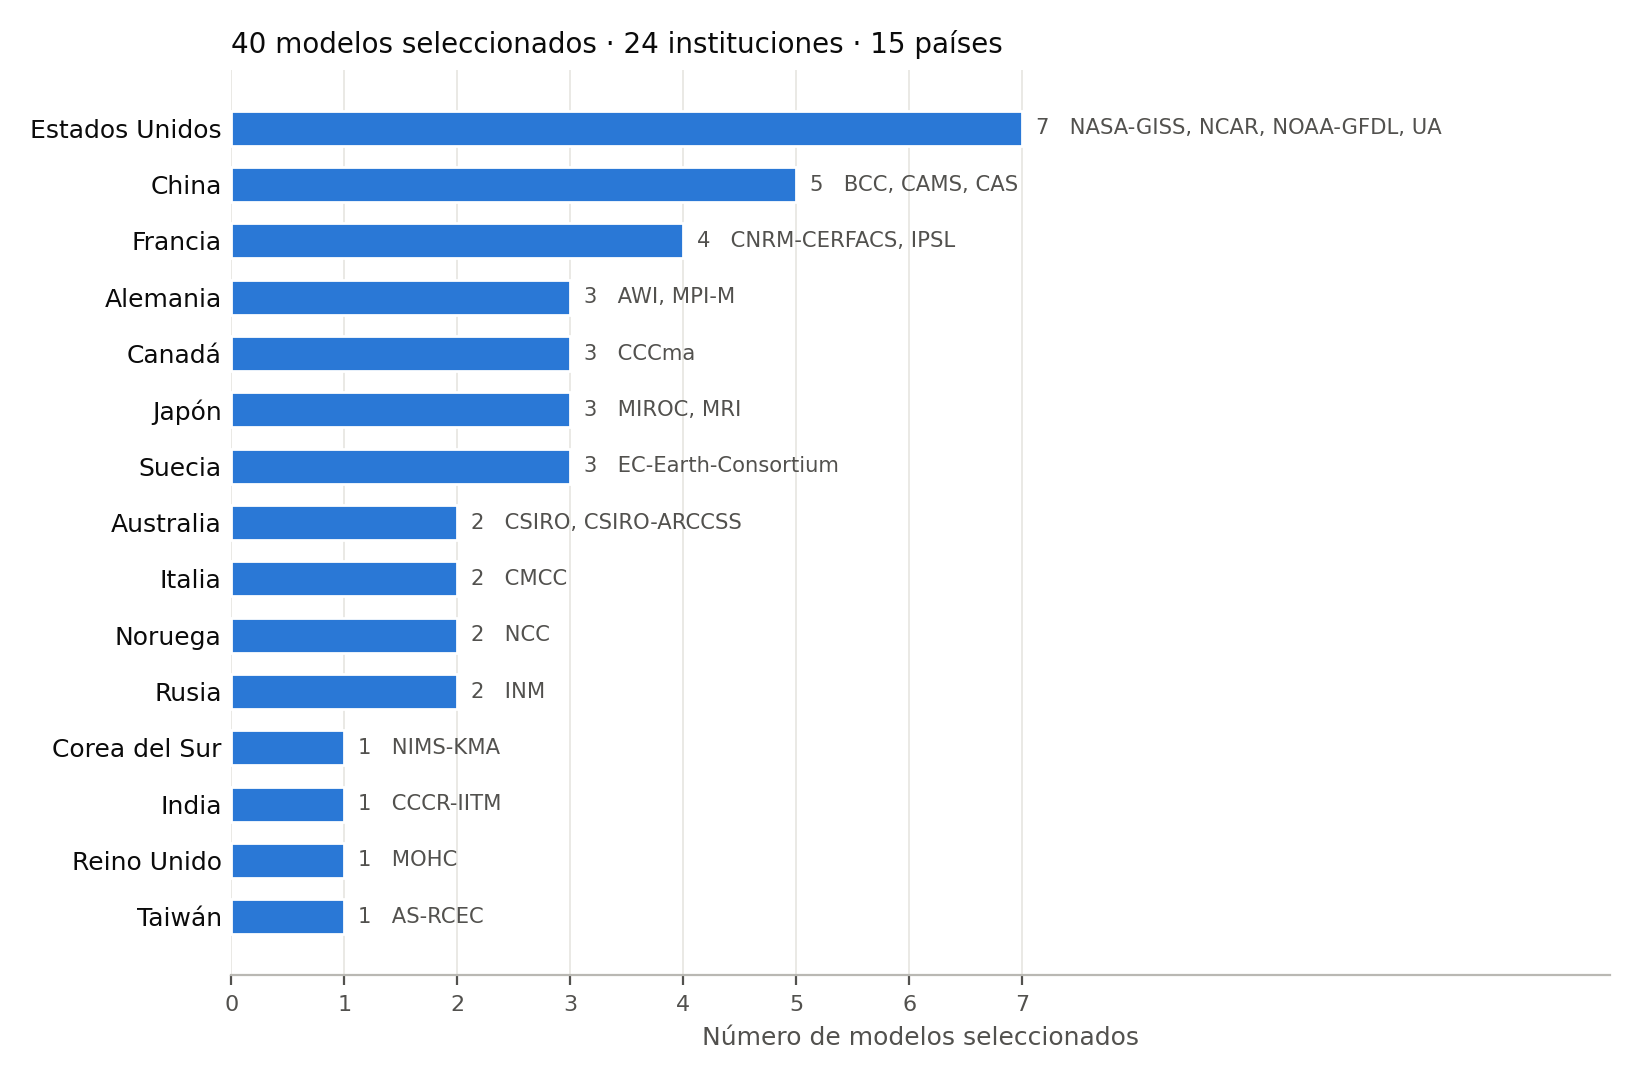
\includegraphics[width=0.92\textwidth]{figuras/contribucion_paises.png}
\caption[Modelos CMIP6 seleccionados por país e institución de origen.]{Modelos CMIP6 seleccionados por país de la institución que los publica, con las instituciones de cada país (fuente: \archivo{informe/model_registry.csv} y \archivo{data/processed/models_inventory_final.csv}). La diversidad de centros de modelado importa para la incertidumbre de modelo: modelos de un mismo centro comparten componentes y, con mayor probabilidad, sesgos estructurales (por ejemplo, la lengua fría o la doble ZCIT del Pacífico oriental), lo que puede reducir artificialmente la dispersión entre modelos.}
\label{fig:cmip6_contribution}
\end{figure}

\subsection{Modelos CMIP6 seleccionados}
\label{sec:tabla_modelos}

El Cuadro~\ref{tab:modelos} lista los 40 modelos seleccionados, con los cuatro experimentos completos y aprobados en el control de calidad (Sección~\ref{sec:resultados}). Cada modelo se identifica con un código \texttt{M001}--\texttt{M102}, asignado alfabéticamente sobre el universo completo de 102 candidatos (\archivo{informe/model_registry.csv}), de modo que un mismo código designa siempre al mismo modelo en cualquier figura o corrida. Las columnas siguen el orden habitual de las tablas de intercomparación CMIP6: primero la identidad del modelo (código, nombre, institución y país) y después sus especificaciones técnicas (miembro de ensamble y resolución nominal). No se incluye una columna de experimentos porque los 40 modelos tienen los mismos cuatro; la disponibilidad por experimento del universo completo se muestra en la Figura~\ref{fig:qc}.

\begingroup\small
\begin{longtable}{@{}L{1.3cm}L{2.9cm}L{3.5cm}L{2.5cm}L{2.1cm}L{\dimexpr\textwidth-12.3cm-10\tabcolsep\relax}@{}}
\caption[Modelos CMIP6 seleccionados: código, institución, país, realización y resolución nominal.]{Modelos CMIP6 seleccionados. Código: identificador estable \texttt{M001}--\texttt{M102}. Institución: \archivo{institution_id} de CMIP6. País: derivado del vocabulario controlado oficial de CMIP6 (\archivo{WCRP-CMIP/CMIP6_CVs}); para consorcios multinacionales como EC-Earth es el país de la sede administrativa. Realización: \archivo{variant_label} común a los cuatro experimentos. Resolución: \archivo{nominal_resolution} de la variante de grilla descargada, la más gruesa entre las que cubren los cuatro experimentos (Sección~\ref{sec:desviacion}); tras el regrillado del Paso~04 todos los modelos comparten la grilla de ERSSTv5 ($\sim$2°).}
\label{tab:modelos} \\
\toprule
\textbf{Código} & \textbf{Modelo} & \textbf{Institución} & \textbf{País} & \textbf{Realización} & \textbf{Resolución} \\
\midrule
\endfirsthead
\toprule
\textbf{Código} & \textbf{Modelo} & \textbf{Institución} & \textbf{País} & \textbf{Realización} & \textbf{Resolución} \\
\midrule
\endhead
\bottomrule
\endfoot
M001 & ACCESS-CM2 & CSIRO-ARCCSS & Australia & r1i1p1f1 & 250\,km \\
M002 & ACCESS-ESM1-5 & CSIRO & Australia & r1i1p1f1 & 250\,km \\
M007 & AWI-CM-1-1-MR & AWI & Alemania & r1i1p1f1 & 25\,km \\
M010 & BCC-CSM2-MR & BCC & China & r1i1p1f1 & 100\,km \\
M012 & CAMS-CSM1-0 & CAMS & China & r1i1p1f1 & 100\,km \\
M013 & CAS-ESM2-0 & CAS & China & r1i1p1f1 & 100\,km \\
M017 & CESM2 & NCAR & Estados Unidos & r1i1p1f1 & 111\,km \\
M019 & CESM2-WACCM & NCAR & Estados Unidos & r1i1p1f1 & 111\,km \\
M023 & CMCC-CM2-SR5 & CMCC & Italia & r1i1p1f1 & 100\,km \\
M025 & CMCC-ESM2 & CMCC & Italia & r1i1p1f1 & 100\,km \\
M026 & CNRM-CM6-1 & CNRM-CERFACS & Francia & r1i1p1f2 & 100\,km \\
M027 & CNRM-CM6-1-HR & CNRM-CERFACS & Francia & r1i1p1f2 & 25\,km \\
M028 & CNRM-ESM2-1 & CNRM-CERFACS & Francia & r1i1p1f2 & 100\,km \\
M029 & CanESM5 & CCCma & Canadá & r1i1p1f1 & 100\,km \\
M030 & CanESM5-1 & CCCma & Canadá & r1i1p1f1 & 100\,km \\
M031 & CanESM5-CanOE & CCCma & Canadá & r1i1p2f1 & 100\,km \\
M038 & EC-Earth3 & EC-Earth-Consortium & Suecia & r1i1p1f1 & 100\,km \\
M043 & EC-Earth3-Veg & EC-Earth-Consortium & Suecia & r1i1p1f1 & 100\,km \\
M044 & EC-Earth3-Veg-LR & EC-Earth-Consortium & Suecia & r1i1p1f1 & 100\,km \\
M051 & FGOALS-f3-L & CAS & China & r1i1p1f1 & 100\,km \\
M052 & FGOALS-g3 & CAS & China & r1i1p1f1 & 100\,km \\
M056 & GFDL-ESM4 & NOAA-GFDL & Estados Unidos & r1i1p1f1 & 111\,km \\
M057 & GISS-E2-1-G & NASA-GISS & Estados Unidos & r1i1p3f1 & 250\,km \\
M059 & GISS-E2-1-H & NASA-GISS & Estados Unidos & r1i1p3f1 & 250\,km \\
M060 & GISS-E2-2-G & NASA-GISS & Estados Unidos & r1i1p3f1 & 250\,km \\
M069 & IITM-ESM & CCCR-IITM & India & r1i1p1f1 & 250\,km \\
M070 & INM-CM4-8 & INM & Rusia & r1i1p1f1 & 100\,km \\
M071 & INM-CM5-0 & INM & Rusia & r1i1p1f1 & 100\,km \\
M074 & IPSL-CM6A-LR & IPSL & Francia & r1i1p1f1 & 100\,km \\
M077 & KACE-1-0-G & NIMS-KMA & Corea del Sur & r1i1p1f1 & 250\,km \\
M079 & MCM-UA-1-0 & UA & Estados Unidos & r1i1p1f2 & 250\,km \\
M081 & MIROC-ES2L & MIROC & Japón & r1i1p1f2 & 111\,km \\
M082 & MIROC6 & MIROC & Japón & r1i1p1f1 & 100\,km \\
M084 & MPI-ESM1-2-HR & MPI-M & Alemania & r1i1p1f1 & 50\,km \\
M085 & MPI-ESM1-2-LR & MPI-M & Alemania & r1i1p1f1 & 250\,km \\
M087 & MRI-ESM2-0 & MRI & Japón & r1i1p1f1 & 100\,km \\
M094 & NorESM2-LM & NCC & Noruega & r1i1p1f1 & 100\,km \\
M095 & NorESM2-MM & NCC & Noruega & r1i1p1f1 & 100\,km \\
M097 & TaiESM1 & AS-RCEC & Taiwán & r1i1p1f1 & 100\,km \\
M100 & UKESM1-0-LL & MOHC & Reino Unido & r1i1p1f2 & 100\,km \\
\end{longtable}
\endgroup

La resolución nominal es una categoría del vocabulario controlado de CMIP6, no una medida continua, y se consulta en el índice de ESGF para la variante de grilla usada por cada modelo (campo \archivo{nominal_resolution}, registrado por el Paso~00b). El miembro de ensamble es \texttt{r1i1p1f1} en 30 de los 40 modelos; en los demás modelos \texttt{r1i1p1f1} no cubre los cuatro experimentos y se usa otra variante común a todos ellos (\texttt{f2}, \texttt{p2} o \texttt{p3}, según el modelo).

\subsection{Selección de modelos}
\label{sec:desviacion}

Como referencia se consideraron los 53 modelos CMIP6 evaluados por \citet{bruno2023} para Sudamérica. El criterio de selección adoptado es más amplio: el script \archivo{00b_build_model_list.py} (Sección~\ref{sec:scripts}) enumera todos los modelos CMIP6 que publican \texttt{tos}/\texttt{Omon} en ESGF (102) y selecciona los que publican los cuatro experimentos requeridos (41). Este criterio tiene dos fundamentos: la selección de \citet{bruno2023} se validó sobre variables atmosféricas continentales y no sobre TSM en Niño~3.4 y Niño~1+2, y un universo más amplio permite que el Entregable~2 decida con datos propios qué modelos representan mejor el ENOS observado, sin descartar candidatos de antemano. Los 53 modelos de \citet{bruno2023} forman parte del universo de 102; 32 de ellos están entre los 40 seleccionados, y los 21 restantes no publican en ESGF alguno de los escenarios requeridos.

Exigir \texttt{ssp370} además de los escenarios del TdR tiene un costo que conviene hacer explícito: 49 modelos publican \texttt{historical}, \texttt{ssp245} y \texttt{ssp585}, y 8 de ellos no publican \texttt{ssp370}, por lo que el requisito del escenario intermedio reduce el conjunto de 49 a 41 modelos. Si en entregables posteriores se prioriza el tamaño del ensamble para SSP2-4.5 y SSP5-8.5, esos 8 modelos pueden incorporarse sin modificar el \emph{pipeline} (Sección~\ref{sec:recomendaciones}).

De cada modelo se descarga la variante de grilla (\archivo{grid_label}) más gruesa entre las que publican los cuatro experimentos, y no la de mayor resolución: como el Paso~04 regrilla todo a la resolución de ERSSTv5 ($\sim$2°), descargar variantes más finas no aportaría precisión al resultado y solo aumentaría el volumen de datos y el tiempo de descarga.

\subsection{Dominios oceanográficos y periodos}
\label{sec:dominios_periodos}

Los dominios se definen en \texttt{config/domains.yaml} en convención de longitud 0--360, usada de forma consistente en todo el \emph{pipeline}:

\begin{itemize}
\item \textbf{Niño~3.4}: 170°O--120°O, 5°S--5°N (190°--240° en 0--360).
\item \textbf{Niño~1+2}: 90°O--80°O, 10°S--0° (270°--280° en 0--360).
\item \textbf{Ventana de descarga}: toda la franja tropical, 0°--360° de longitud y 30°S--30°N.
\end{itemize}

\begin{figure}[htbp]
\centering
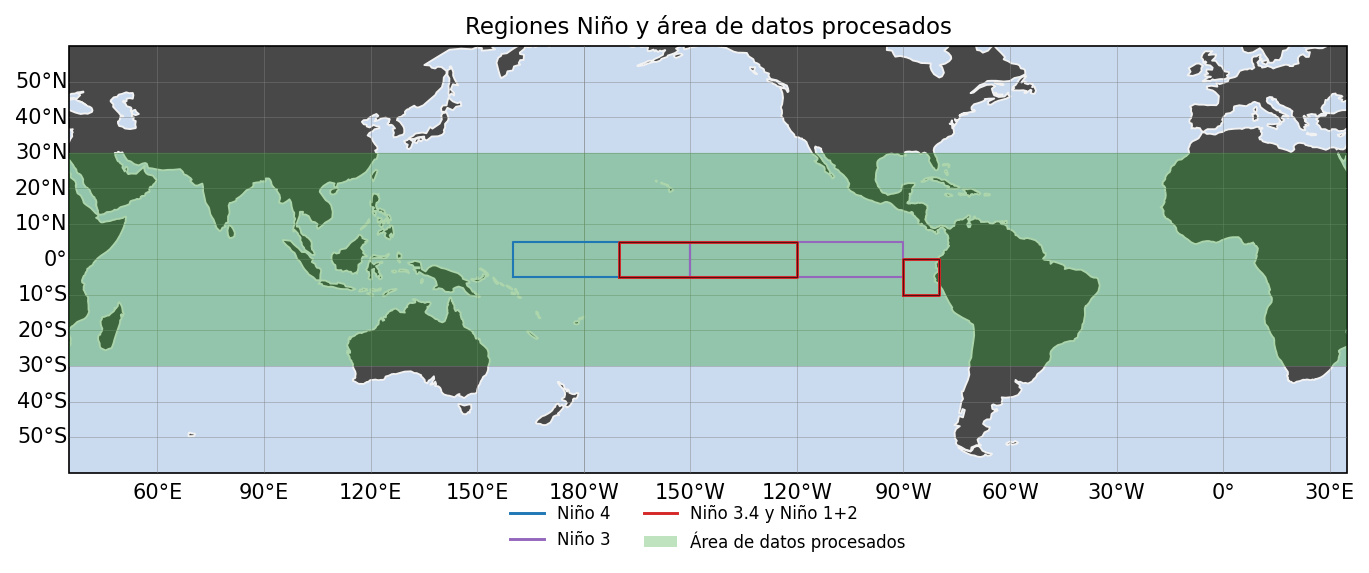
\includegraphics[width=0.9\textwidth]{figuras/region_nino_proj.png}
\caption[Ubicación de las cajas Niño~3.4 y Niño~1+2 y de la ventana de descarga.]{Regiones Niño~3.4 y Niño~1+2 (rojo), con Niño~4 y Niño~3 como referencia, en proyección cilíndrica centrada en Niño~3.4. El área verde es la ventana de descarga (0°--360°, 30°S--30°N): el dominio descargado, regrillado y enmascarado por el \emph{pipeline}. Niño~1+2, junto a la costa peruana y a la surgencia de la Corriente de Humboldt, es la caja de mayor relevancia para el monitoreo del Niño costero \citep{takahashi2019}; Niño~3.4 es la caja de referencia internacional del Índice Oceánico de El Niño (ONI).}
\label{fig:region_nino}
\end{figure}

La ventana cubre toda la franja tropical, y no solo el Pacífico, porque dos cálculos de los entregables siguientes necesitan la TSM media tropical de las tres cuencas: el índice RONI, que expresa la anomalía de Niño~3.4 relativa al promedio tropical, y el índice de calentamiento tropical del método ToD (Sección~\ref{sec:toe_metodos}). Descargar la franja completa en esta etapa evita descargas adicionales en los entregables siguientes.

Los periodos, definidos en \texttt{config/periods.yaml}, son: referencia y validación 1981--2014; proyección 2036--2065 (P1) y 2071--2100 (P2). El rango completo de descarga es 1850--2100 (\texttt{historical}: 1850--2014; escenarios SSP: 2015--2100). Los escenarios son \texttt{ssp245} y \texttt{ssp585}, más \texttt{ssp370} como escenario intermedio para el análisis de sensibilidad entre ambos. El único criterio de selección es la disponibilidad de \texttt{tos}/\texttt{Omon} en los cuatro experimentos.
